\chapter{生命随季节变化}\label{ch:g6:life-through-seasons}

每月初的第一天，给同一棵栗树拍一张照片，
把十二张照片按顺序钉成一排：光秃的枝条、芽、
叶、花穗如烛、栗子、金黄、光秃的枝条，
再一次回到光秃。什么都没有移动——这棵树整年都站在原地——
可一切都变了。\Cref{ch:g3:animals-through-seasons}
追踪了\omterm{def:g1:animals-around-us:animal}{动物}一年中的变化；现在，以测量者的
眼光看整个\omterm{def:g6:exploring-our-environment:components}{环境}，先看\omterm{def:g1:plants-around-us:plant}{植物}。

\section{环境随季节变化}

\begin{proposition}[条件的季节性变化]\label{prop:g6:life-through-seasons:conditions}
一年之中，\omterm{def:g6:exploring-our-environment:components}{环境}的\omterm{def:g6:exploring-our-environment:conditions}{条件}
（\cref{def:g6:exploring-our-environment:conditions}）大幅波动：
白昼时长时短，气温时降时升，
土壤\omterm{def:g6:exploring-our-environment:conditions}{湿度}随雨水与干旱而变化。
一处地点在一月和六月分别调查，
得到的表中两行数据不同——因此，由
\cref{prop:g6:exploring-our-environment:decide}可知，应当预期
两批不同的居住者。
\end{proposition}
\admitted

\begin{example}[同一段树篱，两次调查]\label{ex:g6:life-through-seasons:hedge}
小路边的树篱，调查两次。六月：叶片茂密，
树根处开着十种\omterm{def:g1:plants-around-us:plant}{植物}的花，蜜蜂嗡嗡作响，
黑鸫筑巢，雨后有蜗牛。一月：枝条光秃，
绿色只剩常春藤和\omterm{prop:g4:plants-without-seeds:damp}{苔藓}，没有\omterm{prop:g3:sorting-living-things:groups}{昆虫}飞行，
黑鸫在落叶层中觅食，蜗牛封闭在壳内，
藏在土坡深处。同一地点，同样的成分清单——
\omterm{def:g6:exploring-our-environment:components}{生物}、无机物、痕迹——但\omterm{def:g6:exploring-our-environment:components}{生物}一栏
已经变了模样。
\end{example}

\section{植物如何度过不利的季节}

\begin{definition}[落叶与常绿]\label{def:g6:life-through-seasons:trees}
树木按其对冬季的应对方式分为两类：
\begin{itemize}
  \item \emph{落叶}\index{落叶}树——橡树、
        栗树、山毛榉——秋季落尽全部叶片，
        光秃秃地站立；
  \item \emph{常绿}\index{常绿}树——松树、
        冬青、墙上的常春藤——整个冬天都保持有功能的叶片，
        通常是坚韧、覆有蜡质或呈针状的叶；
        （\cref{prop:g3:sorting-living-things:plants}中
        已提到过针叶）。
\end{itemize}
\end{definition}

\begin{definition}[芽]\label{def:g6:life-through-seasons:buds}
落叶树在冬天并没有死：下一个春天的\omterm{def:g1:plants-around-us:parts}{叶子}
已经以\emph{芽}\index{芽}的形式挤在枝条上——
微小而完整的新枝，叶片折叠得很小，
外面包着防水的鳞片。春天“新”长出的\omterm{def:g1:plants-around-us:parts}{叶子}，
前一年夏天就已经形成了；芽就是为它们储存的冬季仓库。
\end{definition}

\begin{example}[打开一个七叶树的芽]\label{ex:g6:life-through-seasons:bud}
七叶树粘手的大芽，用刀片很容易剖开
（需要大人来做）：在上过清漆般的鳞片之下，
包着绒毛般的棉絮，里面躺着微型的折叠叶片——
完整、苍白、静待时机。二月剪下一段枝条，
插在室内的水中，几周之内就“发芽展叶”了：
枝条里的新枝早已完成，只是缺少\omterm{def:g6:exploring-our-environment:conditions}{温度}。
\end{example}

\begin{omfigure}
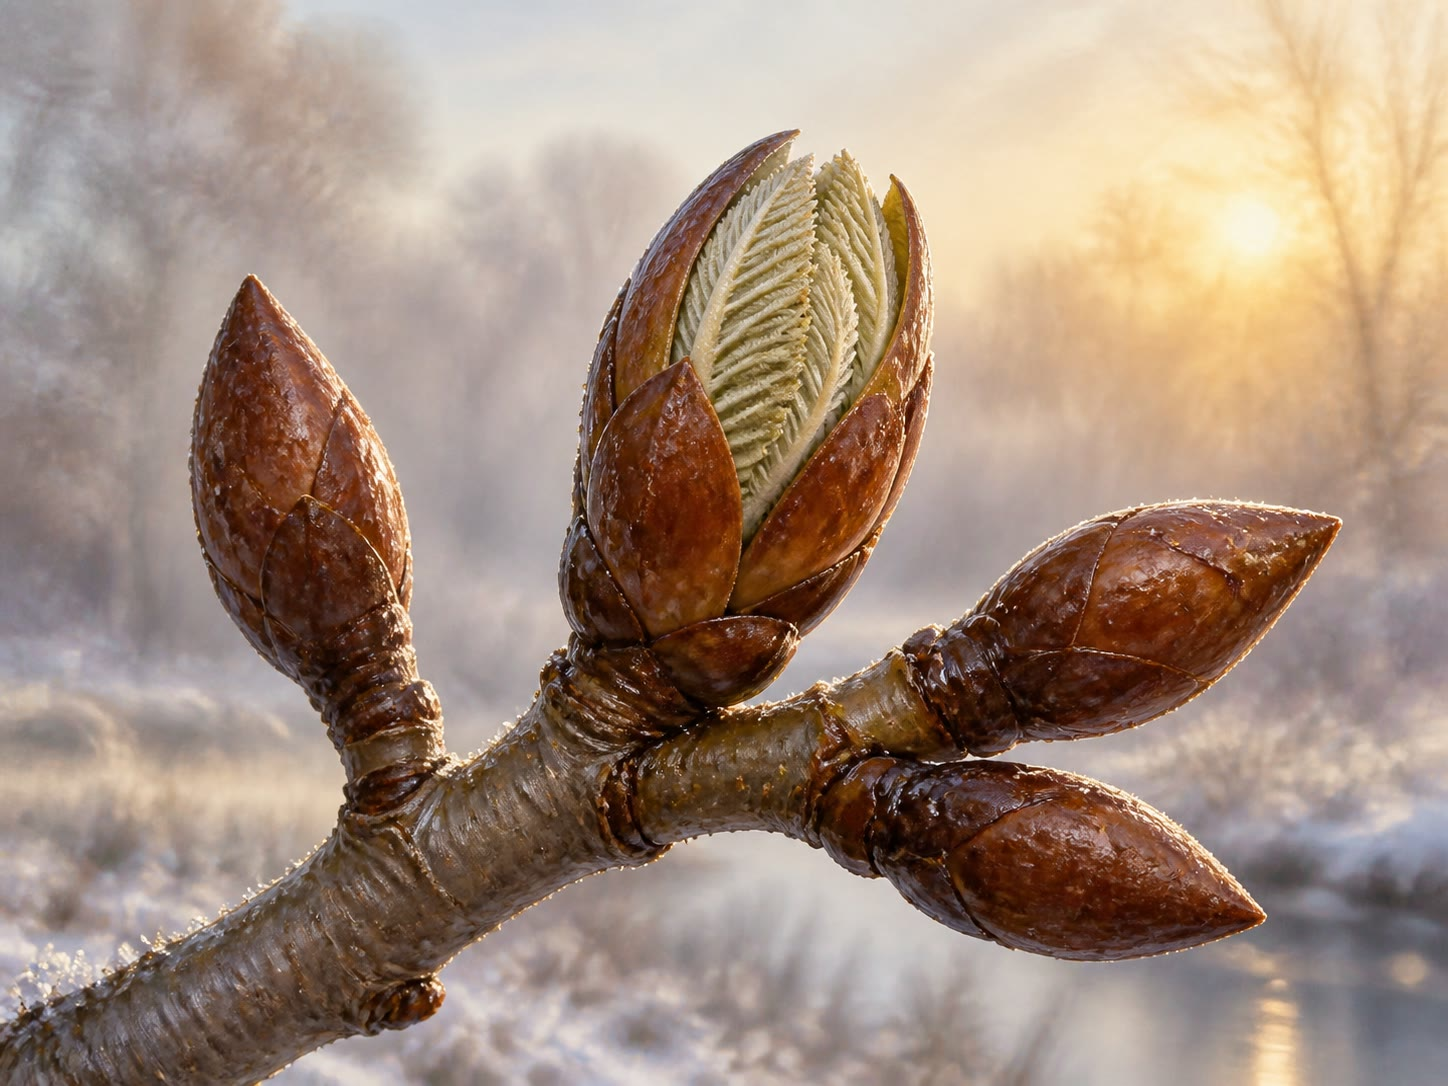
\includegraphics[width=0.56\linewidth]{images/book1/ai/g6-seasons-buds.jpg}

{\small 冬季的仓库，打开之后：七叶树
清漆般的芽鳞之内，下一个春天的\omterm{def:g1:plants-around-us:parts}{叶子}
折叠着，已经完整成形。}
\end{omfigure}

\begin{proposition}[草本层的冬季应对]\label{prop:g6:life-through-seasons:herbs}
较矮的\omterm{def:g1:plants-around-us:plant}{植物}有它们自己的策略：
\begin{itemize}
  \item \emph{一年生植物}\index{一年生植物}——罂粟、菜豆——
        秋季整株死亡，以
        \emph{\omterm{def:g2:from-seed-to-plant:seed}{种子}}的形式度过冬季（\cref{prop:g2:from-seed-to-plant:needs}：
        \omterm{def:g2:from-seed-to-plant:seed}{种子}能安全地熬过寒冷）；
  \item \emph{多年生植物}\index{多年生植物}——水仙、蒲公英——
        地上部分枯萎，
        在地下以\omterm{ex:g4:plants-without-seeds:bulbtuber}{鳞茎}、\omterm{ex:g4:plants-without-seeds:bulbtuber}{块茎}或坚韧的根茎的形式等待，
        （\cref{ex:g4:plants-without-seeds:bulbtuber}的
        贮藏器官，此时正好发挥冬季作用）；
  \item 地表的\omterm{def:g6:life-through-seasons:trees}{常绿}\omterm{def:g1:plants-around-us:plant}{植物}——\omterm{prop:g4:plants-without-seeds:damp}{苔藓}、常春藤——只是
        坚持下来。
\end{itemize}
\end{proposition}
\admitted

\begin{example}[水仙去哪儿了？]\label{ex:g6:life-through-seasons:daffodil}
水仙丛在三月开花，五月变黄，
到七月已经无影无踪——可是
下一个三月，它又会回来，而且更加茂密。整个夏天、秋天和冬天，它都以
\omterm{ex:g4:plants-without-seeds:bulbtuber}{鳞茎}的形式潜伏在草坪之下：\omterm{def:g1:plants-around-us:plant}{植物}从未离开，
只是退回到了贮藏之中。
\end{example}

\section{动物的日历，再看}

\begin{proposition}[动物的应对，用调查的语言来说]\label{prop:g6:life-through-seasons:animals}
\Cref{ch:g3:animals-through-seasons}中的三种策略——
\omterm{def:g3:animals-through-seasons:migration}{迁徙}、\omterm{def:g3:animals-through-seasons:hibernation}{冬眠}、\omterm{def:g3:animals-through-seasons:active}{保持活动}——现在要理解为
对所调查到的变化的应对：每个\omterm{def:g5:biodiversity:species}{物种}都追随其
所需要的\omterm{def:g6:exploring-our-environment:conditions}{条件}和食物。
\begin{itemize}
  \item 燕子追随食物的来源，飞往
        \omterm{def:g6:exploring-our-environment:conditions}{条件}能让\omterm{prop:g3:sorting-living-things:groups}{昆虫}继续飞行的地方；
  \item 刺猬和封闭在壳内的蜗牛，
        等待过完身体无法运转的那些月份；
  \item \omterm{prop:g3:sorting-living-things:groups}{昆虫}提供了第四种应对方式：多数以
        \emph{卵、幼虫或蛹}的形式度过冬季
        （\cref{ex:g2:animals-grow-up:butterfly}），藏在
        土壤、树皮或落叶层之中——成虫死亡，
        \omterm{def:g5:biodiversity:species}{物种}则以其幼体阶段越冬。
\end{itemize}
\end{proposition}
\admitted

\begin{example}[六月的昆虫在一月时身在何处]\label{ex:g6:life-through-seasons:insects}
一月的树篱中不见一只\omterm{prop:g3:sorting-living-things:groups}{昆虫}——而六月的\omterm{prop:g3:sorting-living-things:groups}{昆虫}
却全都在场：蝴蝶化作蛹，藏在压顶石下，
蚱蜢化作卵，埋在土壤中，
瓢虫是挤成一团沉睡的成虫，藏在深深的落叶层中，
蜜蜂则在蜂巢里紧紧聚成一团、保持温暖。六月的调查可以四处走动；
一月的调查却得挖、掀、细看——
这些居民改变的是\emph{形态}，而非住址。
\end{example}

\begin{method}[全年调查]\label{met:g6:life-through-seasons:yearsurvey}
研究一处场地的季节性生命活动时：
\begin{enumerate}
  \item 对同一块做好标记的场地
        进行调查（\cref{met:g6:exploring-our-environment:survey}）
        每季一次——同一方块、同样的仪器、
        同样的搜寻时间；
  \item 每次都要记录\omterm{def:g6:exploring-our-environment:conditions}{条件}\emph{和}居民；
        在同一位置为场地拍照；
  \item 有意寻找冬季隐藏的形态：芽、
        \omterm{ex:g4:plants-without-seeds:bulbtuber}{鳞茎}、卵、蛹、封闭的蜗牛——并
        把所有覆盖物放回原处；
  \item 将四次调查并排摆放：每一处居民的变化
        都要与一次\omterm{def:g6:exploring-our-environment:conditions}{条件}变化相配对，并
        说明每一个缺席者的冬季形态或去向。
\end{enumerate}
\end{method}

\begin{remark}[没有什么会凭空消失]\label{rem:g6:life-through-seasons:vanish}
全年记录的表格揭示了一条深刻的规律：六月调查中的
任何\omterm{def:g5:biodiversity:species}{物种}都不是简单地消失了。它们各自身在别处，
或\omterm{def:g3:animals-through-seasons:migration}{迁徙}，或\omterm{def:g3:animals-through-seasons:hibernation}{冬眠}，或以\omterm{ex:g4:plants-without-seeds:bulbtuber}{鳞茎}、\omterm{def:g2:from-seed-to-plant:seed}{种子}形式储藏，
或处于另一个生命阶段（卵、蛹）。“不见了”
在生物学中从来不是完整的答案，后续的问题
总是：\emph{去了哪里，以什么形式？}
\end{remark}

\section{练习}

\begin{exercise}[$\star$]\label{exo:g6:life-through-seasons:1}
哪些场地\omterm{def:g6:exploring-our-environment:conditions}{条件}会随季节变化？请
列举三项。
\end{exercise}

\begin{exercise}[$\star$]\label{exo:g6:life-through-seasons:2}
判断橡树、松树、山毛榉、冬青、七叶树分别是
落叶还是\omterm{def:g6:life-through-seasons:trees}{常绿}？“落叶”与“\omterm{def:g6:life-through-seasons:trees}{常绿}”各是什么意思？
\end{exercise}

\begin{exercise}[$\star$]\label{exo:g6:life-through-seasons:3}
\omterm{def:g6:life-through-seasons:buds}{冬芽}内部有什么结构？它是何时形成的？
\end{exercise}

\begin{exercise}[$\star$]\label{exo:g6:life-through-seasons:4}
\omterm{prop:g6:life-through-seasons:herbs}{一年生植物}如何度过冬季？
那么像水仙这样的\omterm{prop:g6:life-through-seasons:herbs}{多年生植物}呢？
\end{exercise}

\begin{exercise}[$\star$]\label{exo:g6:life-through-seasons:5}
解释\cref{ex:g6:life-through-seasons:bud}中的二月
枝条：为什么它能在室内提前数周长出\omterm{def:g1:plants-around-us:parts}{叶子}？
\end{exercise}

\begin{exercise}[$\star$]\label{exo:g6:life-through-seasons:6}
列出\omterm{def:g1:animals-around-us:animal}{动物}应对冬季的四种方式，每种各举一个
\omterm{def:g5:biodiversity:species}{物种}为例。
\end{exercise}

\begin{exercise}[$\star\star$]\label{exo:g6:life-through-seasons:7}
对六月树篱中的每一种居民，说出它在一月时的形态和
住址：蝴蝶、蚱蜢、瓢虫、蜗牛、燕子。
\end{exercise}

\begin{exercise}[$\star\star$]\label{exo:g6:life-through-seasons:8}
为什么四次季节性调查必须使用同一场地、
同样的仪器和同样的搜寻时间？
\cref{ch:g6:exploring-our-environment}中的哪条规则在起作用？
\end{exercise}

\begin{exercise}[$\star\star$]\label{exo:g6:life-through-seasons:9}
一月的树篱调查所记录的\omterm{def:g6:exploring-our-environment:components}{生物}数量远少于
六月。请给出两个理由，说明这一差异夸大了
真实的损失，可利用\cref{ex:g6:life-through-seasons:insects}。
\end{exercise}

\begin{exercise}[$\star\star$]\label{exo:g6:life-through-seasons:10}
一位园丁在八月挖开了“死掉的”水仙地块，
发现里面有结实的\omterm{ex:g4:plants-without-seeds:bulbtuber}{鳞茎}。请
结合\cref{prop:g6:life-through-seasons:herbs}解释这一发现：
\omterm{def:g1:plants-around-us:plant}{植物}处于什么状态？\omterm{ex:g4:plants-without-seeds:bulbtuber}{鳞茎}在三月会有什么变化？
\end{exercise}

\begin{exercise}[$\star\star$]\label{exo:g6:life-through-seasons:11}
运用\cref{rem:g6:life-through-seasons:vanish}：一处池塘的
青蛙在一月无处可寻。请给出两个应追问的
问题，并以蟾蜍和青蛙为例说明它们的答案。
\end{exercise}

\begin{exercise}[$\star\star\star$]\label{exo:g6:life-through-seasons:12}
\omterm{def:g6:life-through-seasons:trees}{常绿}\omterm{def:g1:plants-around-us:plant}{植物}的叶质地坚韧、表面有蜡质或呈针状；
落叶\omterm{def:g1:plants-around-us:plant}{植物}的叶则宽而薄。试提出\omterm{def:g6:life-through-seasons:trees}{常绿}叶的结构
能应对冬季的什么问题（可参考鼠妇的失水
问题，但思路相反），以及落叶树为什么
宁可脱落薄薄的\omterm{def:g1:plants-around-us:parts}{叶子}。
\end{exercise}

\section{问题：十二张照片}

\begin{problem}[{周末问题——一棵栗树的一年，
逐帧阅读}]\label{pb:g6:life-through-seasons:1}
莉娜每月初在大门旁为栗树拍一张照片，连拍一年，
并把十二张照片依次钉成一排。
每张照片下方，她都记下当天的昼长和
清晨的\omterm{def:g6:exploring-our-environment:conditions}{温度}。

\medskip\noindent\textbf{第一部分——读懂这一排。}
\begin{enumerate}
  \item 一月和十二月的照片都只见光秃的枝条。在两张照片中，
        枝条上的什么迹象能证明这棵树还活着，
        并且已为春天做好准备？
  \item 芽是在哪两张照片之间展开的？
        莉娜那里的记录写着：昼长
        $11$--$13$ 小时，清晨
        $8$--\qty{12}{\degreeCelsius}。这棵树在回应哪些变化的
        \omterm{def:g6:exploring-our-environment:conditions}{条件}？
  \item 五月的照片中，白色的\omterm{def:g1:plants-around-us:parts}{花朵}排成直立的“蜡烛”，
        依据\cref{ch:g3:flowers-fruits-seeds}（或
        \cref{ch:g5:flower-to-fruit}），五月与九月之间，什么必须前来访花，
        十月的七叶果才会存在？
        七叶果究竟是什么？
  \item 十月的照片中是金黄的\omterm{def:g1:plants-around-us:parts}{叶子}；十一月的照片中，
        枝条光秃，下方铺着一层棕色的落叶。
        依据
        \cref{def:g6:life-through-seasons:trees}，指出这棵树属于哪一类，
        并说明它下一个春天的芽在之后的照片中
        储存在哪里。
\end{enumerate}

\medskip\noindent\textbf{第二部分——树的邻居。}
\begin{enumerate}[resume]
  \item 树下，三月的照片拍到一片水仙，
        它在七月的照片中已经不见。七月时这片水仙
        在哪里，又以什么形式存在？
  \item 六月时小路边开着罂粟花；一月的照片中，
        那里只剩裸露的土壤。一月时罂粟以什么形式存在，
        又采用哪一种策略，
        依据\cref{prop:g6:life-through-seasons:herbs}？
  \item 六月的照片拍到树上方有一只燕子，树下的花上有蜜蜂；
        十一月到二月，两者都不出现。
        请分别说明它们在那段时间里身处何处，
        以什么形式存在。
  \item 喜鹊在每一张照片中都出现。这属于哪种\omterm{def:g1:animals-around-us:animal}{动物}策略，
        喜鹊在整个冬天必须应付什么，
        而燕子只要迁走便可避开的，
        是什么？
\end{enumerate}

\medskip\noindent\textbf{第三部分——这一排的规律。}
\begin{enumerate}[resume]
  \item 莉娜总结道：“树的一年跟随\omterm{def:g6:exploring-our-environment:conditions}{条件}的一年。”
        请用两组配对来支持她的说法：每一组都是
        树在相邻两张照片之间的变化，
        对应她记录的昼长或\omterm{def:g6:exploring-our-environment:conditions}{温度}的变化。
  \item 她的小弟弟说，七月那片水仙
        “死了”这一说法，请用
        \cref{rem:g6:life-through-seasons:vanish}纠正他，
        并说明他说“不见了”时总应追问的
        那个后续问题。
  \item 请详细预测第 13 张照片——即明年一月的照片——
        枝条、小枝和树下的地面。你的预测中，哪些部分
        确定性足够高、值得押注？
        并说明理由。
  \item 二月剪下一枝栗树枝条，插在室内的温水中，
        三周后便长出新叶。这说明
        芽在等待的是\emph{哪一种}\omterm{def:g6:exploring-our-environment:conditions}{条件}？
        请设计一个双枝对照的公平实验，
        见\cref{met:g4:what-plants-need:fairtest}，
        以确定这一点。
\end{enumerate}
\end{problem}
